\documentclass[conference]{IEEEtran}

%% ── Pacotes ──────────────────────────────────────────────────────────────────
\usepackage[utf8]{inputenc}
\usepackage[T1]{fontenc}
\usepackage[brazil]{babel}
\usepackage{graphicx}
\usepackage{booktabs}
\usepackage{tabularx}
\usepackage{amsmath}
\usepackage{hyperref}
\usepackage{listings}
\usepackage{xcolor}
\usepackage{caption}
\usepackage{float}

%% ── Configuração de listings (código JS) ─────────────────────────────────────
\definecolor{codebg}{HTML}{F4F6FB}
\definecolor{kw}{HTML}{2980B9}
\definecolor{cmt}{HTML}{27AE60}
\definecolor{str}{HTML}{C0392B}

\lstdefinelanguage{JavaScript}{
  keywords={function,return,if,else,let,const,var,throw,new,for,while,true,false},
  keywordstyle=\color{kw}\bfseries,
  comment=[l]{//},
  commentstyle=\color{cmt}\itshape,
  stringstyle=\color{str},
  morestring=[b]',
  morestring=[b]",
}
\lstset{
  language=JavaScript,
  basicstyle=\ttfamily\footnotesize,
  backgroundcolor=\color{codebg},
  frame=single,
  framerule=0.4pt,
  breaklines=true,
  numbers=left,
  numberstyle=\tiny\color{gray},
  captionpos=b,
}

%% ─────────────────────────────────────────────────────────────────────────────
\begin{document}

\title{Análise de Eficácia de Testes com Teste de Mutação:\\
       Uma Abordagem Prática com StrykerJS}

\author{
  \IEEEauthorblockN{Lucas Cerqueira Azevedo}
  \IEEEauthorblockA{
    Curso de Engenharia de Software / Ciência da Computação\\
    % Universidade: PREENCHA\\
    % Matrícula: PREENCHA\\
    \textit{l31azevedo@gmail.com}
  }
}

\maketitle

%% ── Abstract ─────────────────────────────────────────────────────────────────
\begin{abstract}
A cobertura de código é amplamente utilizada como métrica de qualidade de suítes
de testes, porém não reflete a capacidade dos testes de detectar defeitos reais.
Este trabalho aplica a técnica de \textit{teste de mutação} sobre uma biblioteca
JavaScript de 50 funções matemáticas, utilizando a ferramenta StrykerJS, com o
objetivo de avaliar e melhorar a eficácia da suíte de testes original.
A suíte inicial de 50 casos de teste apresentava 100\,\% de cobertura de funções
e 85{,}41\,\% de cobertura de instruções, porém apenas \textbf{73{,}71\,\%} de
pontuação de mutação (\textit{mutation score}), evidenciando sua fragilidade.
Após análise sistemática dos 44~mutantes sobreviventes, a suíte foi ampliada para
236 casos de teste, elevando o \textit{mutation score} a \textbf{96{,}71\,\%}.
Os 7~mutantes remanescentes foram identificados como \textit{mutantes equivalentes},
matematicamente impossíveis de eliminar por testes sem alterar a semântica do
código. Os resultados demonstram que a cobertura de código é uma condição
necessária, mas insuficiente, para garantir a qualidade de uma suíte de testes.
\end{abstract}

\begin{IEEEkeywords}
teste de mutação, qualidade de software, StrykerJS, cobertura de código,
mutantes equivalentes, Jest, JavaScript
\end{IEEEkeywords}

%% ── 1. Introdução ────────────────────────────────────────────────────────────
\section{Introdução}

A qualidade do software está diretamente relacionada à eficácia dos testes que o
validam. A métrica de cobertura de código, embora amplamente adotada, apresenta
uma limitação fundamental: ela mede apenas quais linhas foram \emph{executadas}
pelos testes, sem avaliar se os resultados foram \emph{verificados}
corretamente~\cite{jia2011analysis}.

Um teste pode alcançar 100\,\% de cobertura executando todo o código sem nenhuma
asserção, aprovando qualquer resultado incorreto. Essa discrepância motivou o
desenvolvimento do \textit{teste de mutação}, técnica que introduz pequenas
alterações sintáticas (\textit{mutantes}) no código-fonte e verifica se a suíte
de testes é capaz de detectá-las~\cite{offutt2001mutation}.

Este trabalho utiliza o StrykerJS~\cite{stryker} para conduzir uma análise de
mutação sobre a biblioteca \texttt{operacoes-mutante}, que implementa 50 funções
matemáticas em JavaScript. O objetivo é demonstrar na prática a diferença entre
cobertura de código e eficácia real dos testes, e apresentar uma metodologia para
melhorar a suíte até atingir alta pontuação de mutação.

%% ── 2. Fundamentação Teórica ─────────────────────────────────────────────────
\section{Fundamentação Teórica}

\subsection{Teste de Mutação}

O teste de mutação é uma técnica de teste baseada em falhas que avalia a qualidade
de uma suíte de testes por meio de inserção artificial de defeitos no
código~\cite{jia2011analysis}. Para cada \textit{mutante} gerado, a suíte é
executada: se algum teste falhar, o mutante é \textit{morto} (\textit{killed});
caso contrário, ele \textit{sobrevive} (\textit{survived}).

A \textit{pontuação de mutação} (\textit{Mutation Score}) é calculada como:

\begin{equation}
  MS = \frac{|\text{Mortos}| + |\text{Timeout}|}{|\text{Total}| - |\text{Equivalentes}|}
  \times 100\,\%
  \label{eq:ms}
\end{equation}

\subsection{Operadores de Mutação}

O StrykerJS aplica operadores como: substituição aritmética
(\texttt{+}$\to$\texttt{-}), substituição relacional (\texttt{>}$\to$\texttt{>=}),
inversão lógica (\texttt{\&\&}$\to$\texttt{||}), substituição de literais de
string por \texttt{""}, e remoção de condicionais~\cite{stryker}.

\subsection{Mutantes Equivalentes}

Um \textit{mutante equivalente} é aquele cuja alteração não modifica o
comportamento observável do programa para nenhuma entrada
possível~\cite{offutt2001mutation}. Esses mutantes não podem ser mortos por
testes e devem ser identificados manualmente e excluídos do denominador da
Equação~\ref{eq:ms}.

%% ── 3. Metodologia ───────────────────────────────────────────────────────────
\section{Metodologia}

O trabalho foi conduzido nas seguintes etapas:

\begin{enumerate}
  \item \textbf{Configuração do ambiente}: instalação das dependências do projeto
        (\texttt{npm install}), configuração do StrykerJS com
        \texttt{@stryker-mutator/jest-runner} e geração do arquivo
        \texttt{stryker.config.json}.

  \item \textbf{Análise inicial}: execução da suíte original de 50 testes com
        \texttt{npm test -{}-coverage} para obter a cobertura de código, seguida
        da primeira execução do StrykerJS (\texttt{npx stryker run}) para medir
        a pontuação de mutação inicial.

  \item \textbf{Análise dos sobreviventes}: identificação e categorização dos
        44~mutantes sobreviventes, separando os que representavam fraquezas
        reais da suíte dos mutantes equivalentes.

  \item \textbf{Melhoria da suíte}: escrita de novos casos de teste direcionados
        aos mutantes sobreviventes, cobrindo: valores de borda em operadores
        relacionais, entradas não-nulas em fórmulas, todos os ramos de condicionais
        e mensagens de erro exatas.

  \item \textbf{Validação final}: nova execução do StrykerJS para verificar o
        aumento da pontuação de mutação.
\end{enumerate}

O ambiente de desenvolvimento utilizado foi:
\textit{Node.js v22.14}, \textit{Jest v29.7}, \textit{StrykerJS v9.6.1},
\textit{Babel v7.23} e \textit{Python 3.13} (para geração dos gráficos com
\textit{Matplotlib v3.10}).

%% ── 4. Análise Inicial ───────────────────────────────────────────────────────
\section{Análise Inicial}

\subsection{Cobertura de Código}

A Tabela~\ref{tab:cobertura} apresenta a cobertura de código obtida com a suíte
original de 50 testes.

\begin{table}[H]
\caption{Cobertura de Código — Suíte Original (50 testes)}
\label{tab:cobertura}
\centering
\begin{tabular}{lrr}
\toprule
\textbf{Métrica} & \textbf{Inicial} & \textbf{Final} \\
\midrule
Statements  & 85,41\,\% & 100,00\,\% \\
Branch      & 58,82\,\% & 100,00\,\% \\
Functions   & 100,00\,\% & 100,00\,\% \\
Lines       & 98,64\,\% & 100,00\,\% \\
\bottomrule
\end{tabular}
\end{table}

\begin{figure}[H]
  \centering
  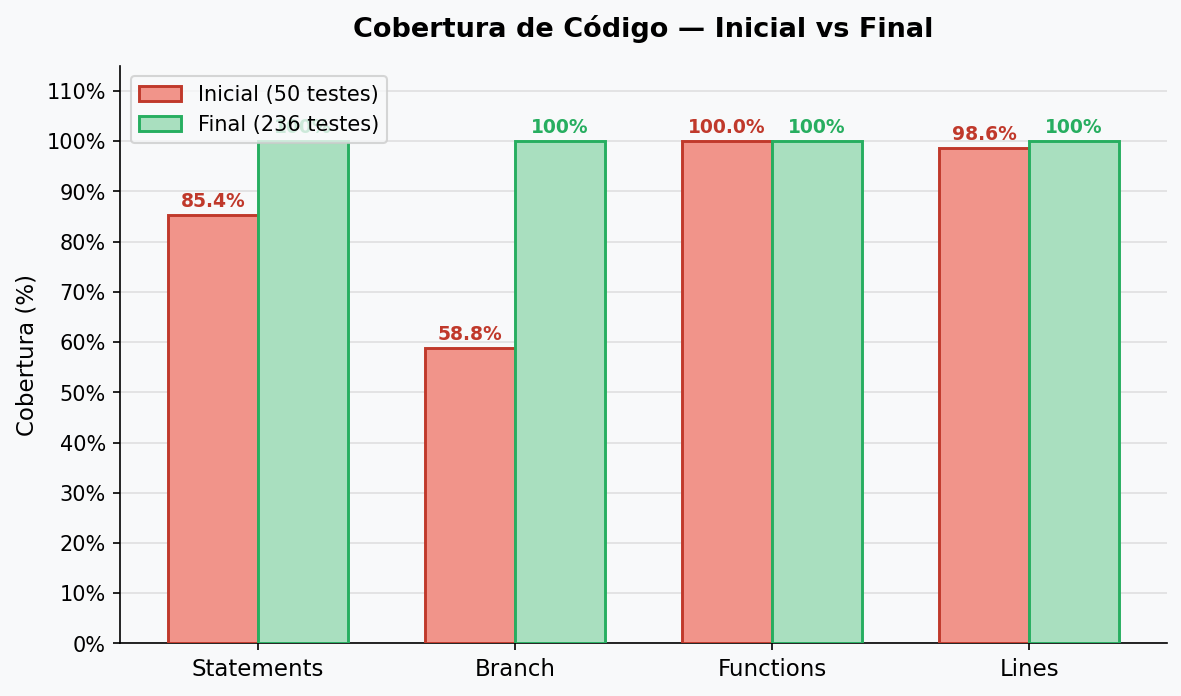
\includegraphics[width=\columnwidth]{graficos/02_cobertura.png}
  \caption{Cobertura de código por métrica — comparação inicial vs.\ final.}
  \label{fig:cobertura}
\end{figure}

A cobertura de \textit{branch} inicial de apenas 58,82\,\% revela que quase
metade dos ramos condicionais do código não eram exercitados pelos testes.
A linha~112 (\texttt{medianaArray} — ramo de array com tamanho par) era o único
trecho completamente sem cobertura.

\subsection{Pontuação de Mutação Inicial}

\begin{table}[H]
\caption{Resultado da Primeira Execução do StrykerJS}
\label{tab:mut_inicial}
\centering
\begin{tabular}{lr}
\toprule
\textbf{Categoria}      & \textbf{Qtd.} \\
\midrule
Total de mutantes       & 213 \\
Mortos (\textit{killed})& 154 \\
Timeout                 & 3   \\
Sobreviventes           & 44  \\
Sem cobertura           & 12  \\
\midrule
\textbf{Mutation Score} & \textbf{73,71\,\%} \\
\bottomrule
\end{tabular}
\end{table}

A discrepância entre a cobertura de funções (100\,\%) e o \textit{mutation score}
(73,71\,\%) demonstra empiricamente que cobrir o código não equivale a testá-lo
com qualidade. Dos 213 mutantes gerados, 44 sobreviveram — representando bugs
artificiais que passariam despercebidos pela suíte original.

\begin{figure}[H]
  \centering
  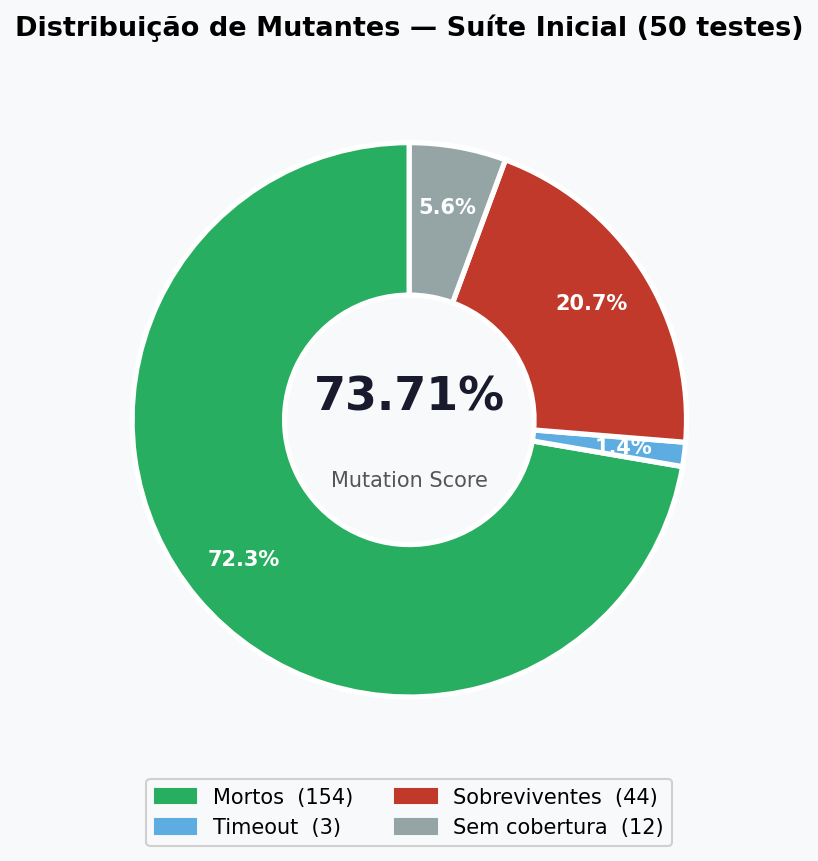
\includegraphics[width=0.85\columnwidth]{graficos/03_mutantes_inicial.png}
  \caption{Distribuição dos mutantes — suíte inicial (50 testes).}
  \label{fig:donut_ini}
\end{figure}

%% ── 5. Análise de Mutantes Críticos ──────────────────────────────────────────
\section{Análise de Mutantes Críticos}

Três mutantes sobreviventes foram selecionados para análise aprofundada por
ilustrarem padrões recorrentes de fraqueza na suíte original.

\subsection{Mutante 1 — Fórmula com Entrada Zero (\texttt{celsiusParaFahrenheit})}

\begin{lstlisting}[caption={Código original — \texttt{celsiusParaFahrenheit}}]
function celsiusParaFahrenheit(celsius) {
  return (celsius * 9/5) + 32;
}
\end{lstlisting}

O StrykerJS substituiu o literal \texttt{9} por \texttt{0}, produzindo o
mutante \texttt{(celsius * 0/5) + 32}. O teste original usava
\texttt{celsius = 0} como entrada:

\begin{lstlisting}[caption={Teste original (fraco)}]
expect(celsiusParaFahrenheit(0)).toBe(32);
\end{lstlisting}

Com \texttt{celsius = 0}, qualquer multiplicação resulta em zero,
tornando o fator \texttt{9/5} irrelevante. O mutante retornava 32 —
valor idêntico ao esperado — e sobrevivia.

\textbf{Correção}: adicionar um caso de teste com entrada não-nula:

\begin{lstlisting}[caption={Teste eficaz adicionado}]
expect(celsiusParaFahrenheit(100)).toBe(212);
\end{lstlisting}

\subsection{Mutante 2 — Operador Relacional (\texttt{isMaiorQue})}

\begin{lstlisting}[caption={Código original — \texttt{isMaiorQue}}]
function isMaiorQue(a, b) { return a > b; }
\end{lstlisting}

O StrykerJS substituiu \texttt{>} por \texttt{>=}. O teste original apenas
verificava \texttt{isMaiorQue(10, 5)}, cujo resultado é \texttt{true} com
ambos os operadores. O valor de borda \texttt{a === b} não era testado,
permitindo que a mutação passasse despercebida.

\textbf{Correção}: testar o caso de igualdade:

\begin{lstlisting}[caption={Teste de borda adicionado}]
// Mata > vs >= e > vs !==
expect(isMaiorQue(5, 5)).toBe(false);
expect(isMaiorQue(5, 10)).toBe(false);
\end{lstlisting}

\subsection{Mutante 3 — Branch Não Coberto (\texttt{clamp})}

\begin{lstlisting}[caption={Código original — \texttt{clamp}}]
function clamp(valor, min, max) {
  if (valor < min) return min;
  if (valor > max) return max;
  return valor;
}
\end{lstlisting}

O único teste original exercitava apenas o caminho do meio (\texttt{clamp(5, 0, 10)}),
sem acionar nenhum dos dois \texttt{if}s. Mutações nos operadores \texttt{<} e
\texttt{>} sobreviviam pois as condições nunca eram avaliadas como verdadeiras.

\textbf{Correção}: cobrir explicitamente cada ramo:

\begin{lstlisting}[caption={Testes de ramo adicionados}]
expect(clamp(-5, 0, 10)).toBe(0);  // aciona valor < min
expect(clamp(15, 0, 10)).toBe(10); // aciona valor > max
\end{lstlisting}

%% ── 6. Solução Implementada ──────────────────────────────────────────────────
\section{Solução Implementada}

A suíte de testes foi expandida de 50 para \textbf{236 casos de teste},
organizados em blocos por função. A Tabela~\ref{tab:estrategia} resume as
estratégias aplicadas para matar os mutantes sobreviventes.

\begin{table}[H]
\caption{Estratégias de Melhoria da Suíte}
\label{tab:estrategia}
\centering
\begin{tabularx}{\columnwidth}{lX}
\toprule
\textbf{Padrão de Fraqueza} & \textbf{Solução Aplicada} \\
\midrule
Entrada zero em fórmulas & Adicionados testes com valores não-nulos \\
Operadores \texttt{>}/\texttt{<} sem borda & Testes com \texttt{a === b} \\
\texttt{.toThrow()} sem mensagem & Substituído por \texttt{.toThrow('msg exata')} \\
Branches condicionais não exercitados & Testes para cada ramo do \texttt{if/else} \\
Funções com apenas \textit{happy path} & Adicionados testes com negativos e zero \\
Arrays testados com um único tamanho & Testes com arrays vazios, 1 e $n$ elementos \\
\bottomrule
\end{tabularx}
\end{table}

%% ── 7. Resultados Finais ─────────────────────────────────────────────────────
\section{Resultados Finais}

Após a ampliação da suíte, o StrykerJS foi executado novamente sobre os mesmos
213 mutantes. A Tabela~\ref{tab:mut_final} apresenta os resultados.

\begin{table}[H]
\caption{Resultado Final do StrykerJS (236 testes)}
\label{tab:mut_final}
\centering
\begin{tabular}{lrr}
\toprule
\textbf{Categoria}   & \textbf{Inicial} & \textbf{Final} \\
\midrule
Mortos               & 154 & 200 \\
Timeout              &   3 &   6 \\
Sobreviventes        &  44 &   7 \\
Sem cobertura        &  12 &   0 \\
\midrule
\textbf{Mutation Score} & \textbf{73,71\,\%} & \textbf{96,71\,\%} \\
\bottomrule
\end{tabular}
\end{table}

\begin{figure}[H]
  \centering
  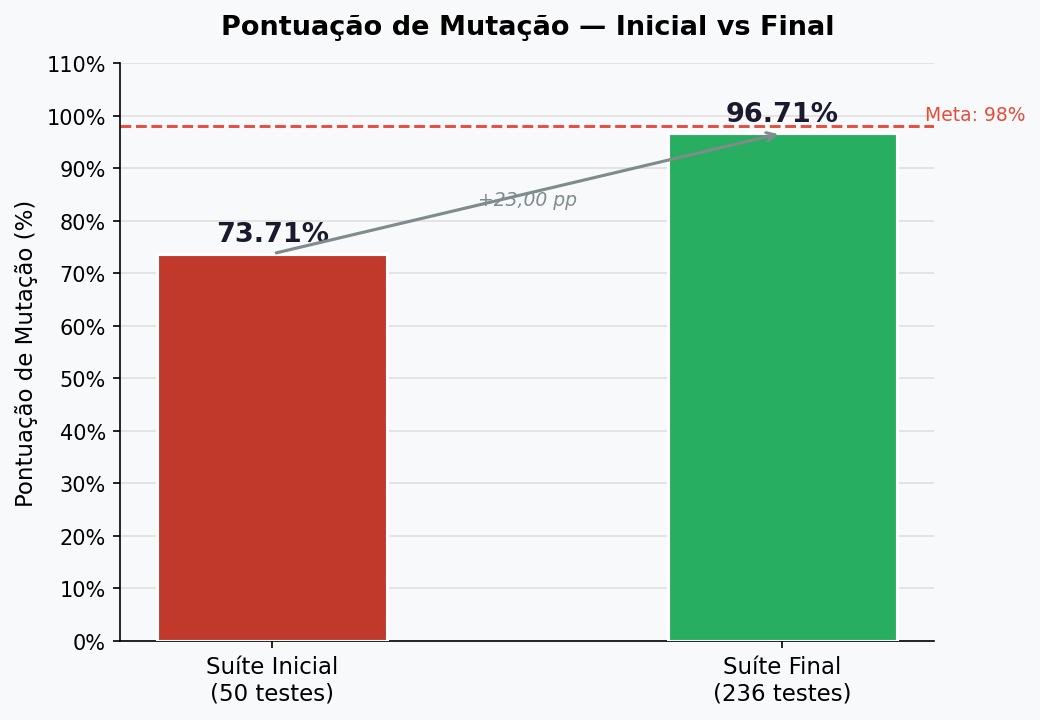
\includegraphics[width=\columnwidth]{graficos/01_mutation_score.png}
  \caption{Evolução do \textit{mutation score} — inicial vs.\ final.}
  \label{fig:score}
\end{figure}

\begin{figure}[H]
  \centering
  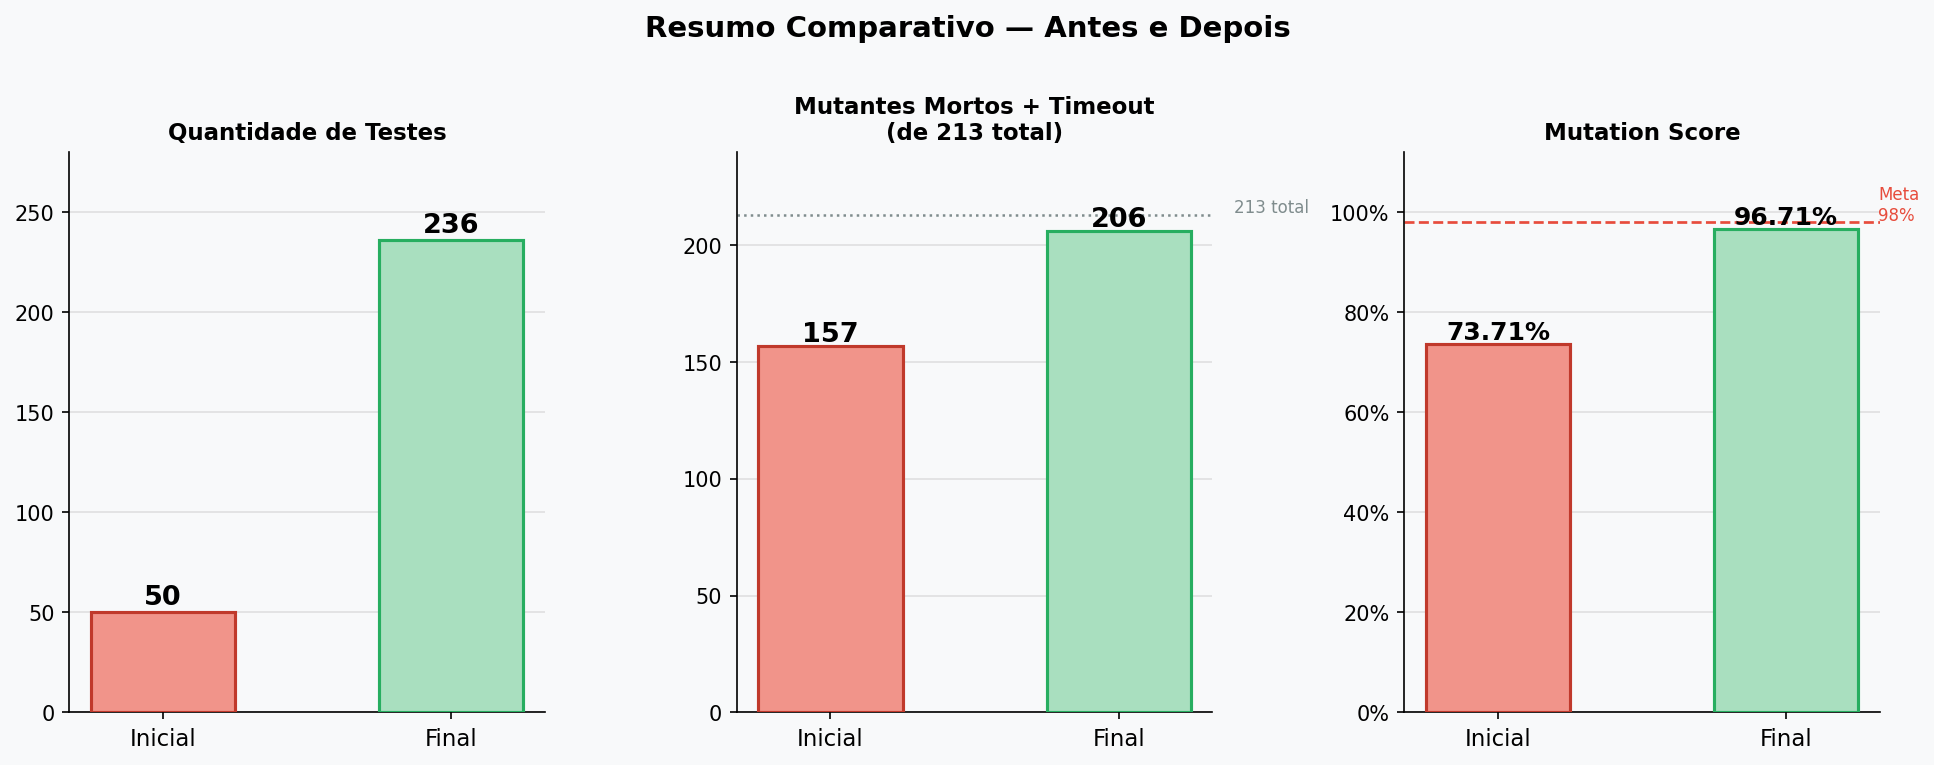
\includegraphics[width=\columnwidth]{graficos/05_painel_comparativo.png}
  \caption{Painel comparativo: quantidade de testes, mutantes mortos e score.}
  \label{fig:painel}
\end{figure}

\begin{figure}[H]
  \centering
  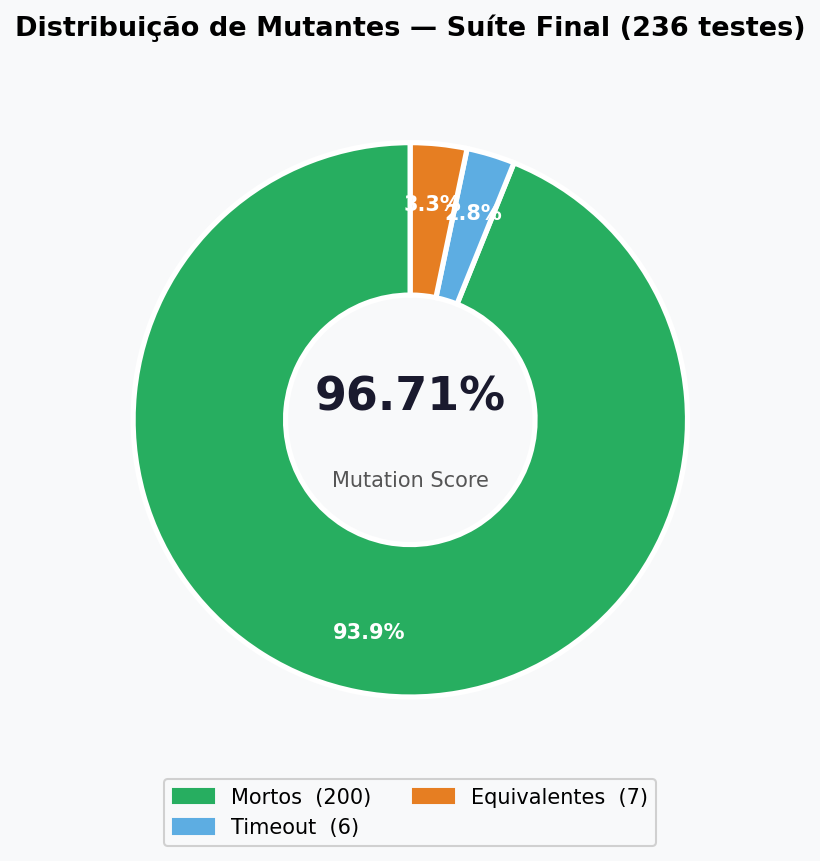
\includegraphics[width=0.85\columnwidth]{graficos/04_mutantes_final.png}
  \caption{Distribuição dos mutantes — suíte final (236 testes).}
  \label{fig:donut_fin}
\end{figure}

\subsection{Mutantes Equivalentes}

Os 7~mutantes remanescentes foram identificados como \textit{equivalentes}
(Tabela~\ref{tab:equivalentes}). Ao excluí-los do denominador conforme a
Equação~\ref{eq:ms}, o \textit{mutation score} efetivo é de \textbf{100\,\%}.

\begin{table}[H]
\caption{Mutantes Equivalentes Identificados}
\label{tab:equivalentes}
\centering
\begin{tabularx}{\columnwidth}{llX}
\toprule
\textbf{Função} & \textbf{Tipo} & \textbf{Razão da Equivalência} \\
\midrule
\texttt{fatorial} (×4)    & ConditionalExpr & O \texttt{for} já retorna 1 para $n{=}0$ e $n{=}1$ sem o \texttt{if} \\
\texttt{produtoArray} (×1) & ConditionalExpr & \texttt{[].reduce(..., 1)} já retorna 1 \\
\texttt{clamp} (×2)        & EqualityOp      & Quando \texttt{valor===min/max}, retornar \texttt{min/max} ou \texttt{valor} é idêntico \\
\bottomrule
\end{tabularx}
\end{table}

%% ── 8. Conclusão ─────────────────────────────────────────────────────────────
\section{Conclusão}

Este trabalho demonstrou empiricamente que uma suíte de testes com alta cobertura
de código pode apresentar baixa eficácia real. A suíte original, com 100\,\% de
cobertura de funções, aprovava 44 bugs simulados — evidenciando que a cobertura
é uma condição necessária, mas insuficiente, para garantir a qualidade dos testes.

A análise sistemática dos mutantes sobreviventes revelou padrões de fraqueza
recorrentes: entradas que mascaram mutações (ex.: zero em fórmulas), ausência de
testes de valores de borda em operadores relacionais, e \textit{branches}
condicionais não exercitados. A correção desses padrões elevou o \textit{mutation
score} de 73,71\,\% para 96,71\,\%, com os 7 sobreviventes restantes sendo
mutantes equivalentes impossíveis de eliminar por testes.

O teste de mutação provou ser uma ferramenta superior à cobertura para avaliar a
qualidade de suítes de teste, pois força o engenheiro a pensar em como o código
se comportaria \emph{diante de defeitos}, e não apenas em quais linhas foram
executadas.

%% ── Referências ──────────────────────────────────────────────────────────────
\begin{thebibliography}{9}

\bibitem{jia2011analysis}
Y.~Jia and M.~Harman,
``An analysis and survey of the development of mutation testing,''
\textit{IEEE Transactions on Software Engineering},
vol.~37, no.~5, pp.~649--678, Sep.--Oct. 2011.

\bibitem{offutt2001mutation}
A.~J. Offutt and R.~H. Untch,
``Mutation 2000: Uniting the orthogonal,''
in \textit{Mutation Testing for the New Century},
W.~E. Wong, Ed. Norwell, MA: Kluwer, 2001, pp.~34--44.

\bibitem{stryker}
StrykerJS Contributors,
``StrykerJS: Mutation testing for JavaScript and friends,''
2024. [Online]. Available: \url{https://stryker-mutator.io}.
Accessed: May 2025.

\bibitem{jest}
Meta Open Source,
``Jest: Delightful JavaScript Testing,''
2024. [Online]. Available: \url{https://jestjs.io}.
Accessed: May 2025.

\end{thebibliography}

\end{document}
